\documentclass[cn,table]{elegantbook}

\usepackage{tikz}
\usepackage{graphicx}
\usepackage{subcaption}
\usepackage[ruled,linesnumbered,vlined]{algorithm2e}
\usepackage{hyperref}
\usepackage{listings}
\usepackage{interval}
\usepackage{xcolor}
\usepackage{ulem}
\usepackage{wrapfig}

\intervalconfig{%
	soft open fences,
}

\def\figureautorefname{图}
\def\sectionautorefname{小节}

\SetAlgorithmName{算法}{算法}{算法索引}

\renewcommand*{\lstlistingname}{代码}

\title{何老师算法课笔记}
\subtitle{Always be patient, sharp and diligent.}
\author{计卓1801全体}
\institute{华中科技大学}
\date{\zhtoday}
\version{1.8.0}
\logo{logo.png}
\cover{cover.png}

\begin{document}
\maketitle
\tableofcontents
\pagenumbering{arabic}

% add your code here
% \input{src/example.tex}
\input{src/Ln1-AsymptoticOrderGrowth.tex}
\input{src/Tiling-Problem.tex}
\input{src/stable-matching.tex}
\chapter{图算法之最小生成树}

\begin{introduction}
	\item 问题概述
	\item Prim算法
	\item Kruskal算法
\end{introduction}

\section{概述}
给定一张边带权的无向图G=(V, E),其中V表示图中点的集合,E表示图中边的集合,n=|V|,m=|E|。
由V中的全部n个顶点和E中n-1条边构成的无向连通子图被称为G的一棵生成树,其中边的权值之和最小的生成树被称为无向图G的最小生成树。

最小生成树最为经典的两个算法分别是Prim算法和Kruskal算法。本节将首先讨论这两个算法的执行过程。

\section{基本概念}
在深入探讨之前,还需明白一些定义:

\begin{definition}{path}{path}
	A path is a sequence of edges which connects a sequence of nodes.
\end{definition}

\begin{definition}{cycle}{cycle}
	A cycle is a path with no repeated nodes or edges other than the
starting and ending nodes.
\end{definition}

可以借助\autoref{fig:path-cycle}理解path以及cycle的概念。

\begin{figure}[hbt]
	\centering
	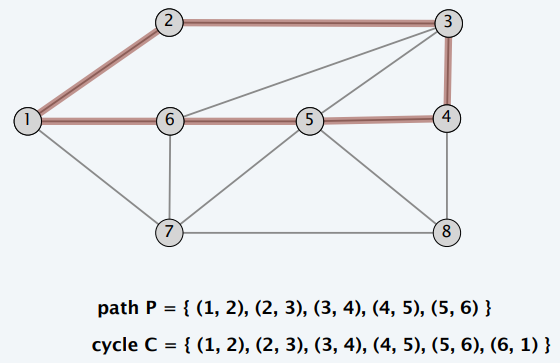
\includegraphics[scale=0.5]{image/pathcycle.png}
	\caption{具体例子说明path和cycle}\label{fig:path-cycle}
\end{figure}

\begin{definition}{cut}{MSTcut}
	A cut is a partition of the nodes into two nonempty subsets S and V / S.
\end{definition}

\begin{definition}{cutset}{MSTcutset}
	The cutset of a cut S is the set of edges with exactly one endpoint in S.
\end{definition}

可以借助\autoref{fig:cut-cutset}理解cut以及cutset的概念。

\begin{figure}[hbt]
	\centering
	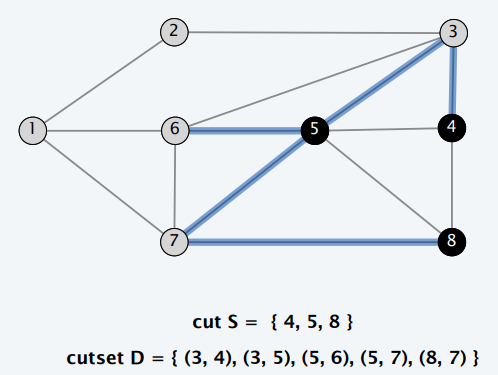
\includegraphics[scale=0.5]{image/cutcutset.png}
	\caption{具体例子说明cut与cutset}\label{fig:cut-cutset}
\end{figure}

\begin{theorem}{}{cycle-cutset-theorem}
	A cycle and a cutset intersect in an even number of edges.
\end{theorem}

可以借助\autoref{fig:cycle-cutset}理解\autoref{cycle-cutset-theorem}。

\begin{figure}[hbt]
	\centering
	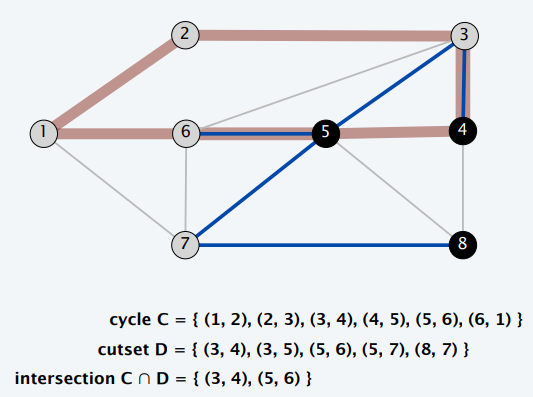
\includegraphics[scale=0.5]{image/cyclecutset.png}
	\caption{cycle、cutset的性质}\label{fig:cycle-cutset}
\end{figure}

\begin{definition}{生成树}{ST}
Let H = (V, T) be a subgraph of an undirected graph G = (V, E).
H is a spanning tree of G if H is both acyclic and connected.
\end{definition}

一个生成树的例子如\autoref{fig:exampleofST}所示。

\begin{figure}[hbt]
	\centering
	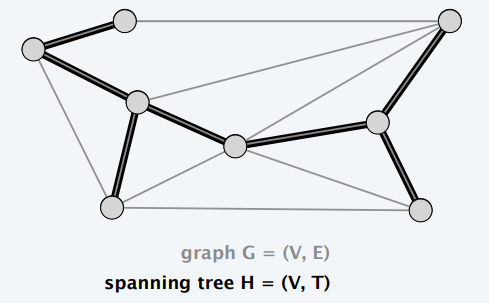
\includegraphics[scale=0.5]{image/exampleofST.png}
	\caption{生成树的例子}\label{fig:exampleofST}
\end{figure}

\begin{theorem}{}{ST-theorem}
	如果H = (V, T)是一个无向图G = (V, E)的子图,那么,以下各条件等价:
	\begin{enumerate}
		\item H是G的一棵生成树
		\item H是无环且连通的
		\item H是连通的并且有 V – 1条边
		\item H是无环的并且有 V – 1条边
		\item 任意拿掉H的一条边,就不再使其连通
		\item 任意增加一条边,则H就会构成环
	\end{enumerate}

\end{theorem}

\begin{definition}{最小生成树}{MST}
	Given a connected, undirected graph G = (V, E) with edge costs $c_e$,
a minimum spanning tree (V, T) is a spanning tree of G such that the sum
of the edge costs in T is minimized.
\end{definition}

一个生成树的例子如\autoref{fig:exampleofMST}所示。

\begin{figure}[hbt]
	\centering
	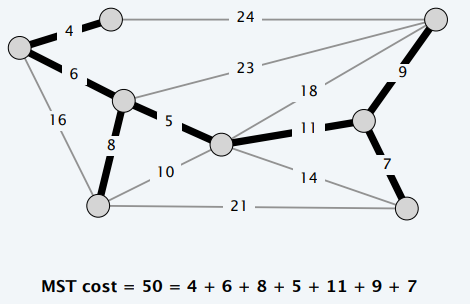
\includegraphics[scale=0.5]{image/exampleofMST.png}
	\caption{生成树的例子}\label{fig:exampleofMST}
\end{figure}

\begin{theorem}{Cayley’s theorem}{Cayley-theorem}
	The complete graph on n nodes has $n^(n–2)$ spanning trees
\end{theorem}

最小生成树是一个基础却有着十分广泛的应用的问题,之后的\autoref{sec:prim}和\autoref{sec:kruskal}
将分别介绍求解最小生成树的Prim算法和Kruskal算法。

\section{Prim算法}\label{sec:prim}
\subsection{算法描述与演示}
\begin{algorithm}
	\DontPrintSemicolon
	\KwIn{Graph G}
	\KwResult{MST of Graph G}
	\Begin{
		$S \leftarrow \{ s \} $ for any node s,$T \leftarrow \emptyset$;\\
		\For{$|T| < n-1$}{
			Add to T a min-weight edge with exactly one endpoint in S;\\
			Add the other endpoint to S;\\
		}
		Return T ;\\
	}
	\caption{Prim}\label{alg:Prim}
\end{algorithm}

算法执行流程如\autoref{fig:Prim}所示。

\begin{figure}[hbt]
	\centering
	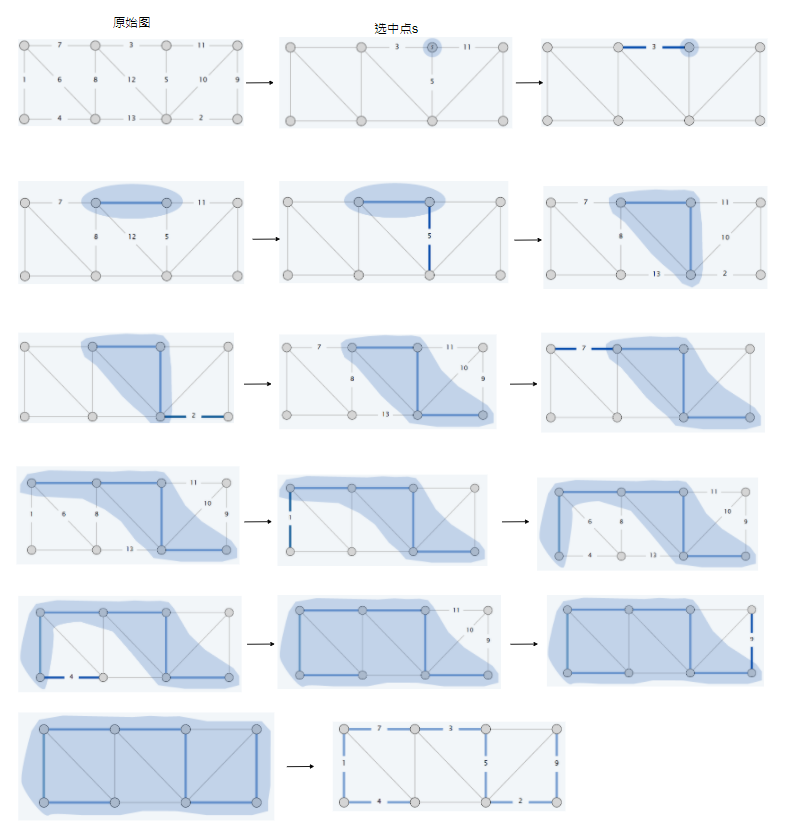
\includegraphics[scale=0.5]{image/prim.png}
	\caption{Prim算法的执行流程}\label{fig:Prim}
\end{figure}

\subsection{算法正确性证明}
记图G是一个连通图,Y是对p使用prim算法得到的一棵生成树,$Y_1$是p的一棵最小生成树
\begin{enumerate}
	\item 若Y=$Y_1$,显然prim算法是正确的
	\item 若Y≠$Y_1$,可进行如下推导:

	a)Y中有$n( n \geq 1 )$条边不存在于$Y_1$中,在构建Y的过程中,第一次遇到这样的一条边时(以e表示),
	则e的一个端点u落在V内(V是之前的prim运算得到的一个子顶点集),另一个端点v落在V外
	
	b)$Y_1$是连通的,故$Y_1$中存在u到v的一条的路径,此路径上必然存在一条边f,它的一个端点落在V内,另一个端点落在V外
	
	c)把e加入$Y_1$,去掉f,$Y_1$仍然连通,根据prim算法,权值$W(f) \geq W(e)$,否则e不会被选入V,
	如果$W(f)>W(e)$,新构建的树的权值和会比$Y_1$小,而$Y_1$是最小生成树,因此$W(f)>W(e)$不成立,得$W(f)=W(e)$
	
	d)对每一条类似e的边,重复过程c),最终Y和重新构建的的$Y_1$拥有的边完全一致,
	新构建的$Y_1$也是最小生成树,因此Y也是最小生成树,证明prim算法正确
\end{enumerate}

\subsection{算法复杂度}
普通堆优化的 Prim 算法复杂度为 $O(mlogn)$,而斐波那契堆优化的 Prim 算法
能达到 $O(m+nlogn)$

\section{Kruskal算法}\label{sec:kruskal}
\subsection{算法描述与演示}
\begin{algorithm}
	\DontPrintSemicolon
	\KwIn{Graph G}
	\KwResult{MST of Graph G}
	\Begin{
		$T \leftarrow \emptyset$;\\
		$S \leftarrow$sort edges by weight;\\
		\While{$e \in S$}{
			\If{$T \cup \{ e \}$ no cycle}{
				$T = T \cup \{ e \};$
			}
			\If{$|T| < n-1$}{
				Return T ;\\
			}
		}
	}
	\caption{kruskal}\label{alg:kruskal}
\end{algorithm}

算法执行流程如\autoref{fig:kruskal}所示。

\begin{figure}[hbt]
	\centering
	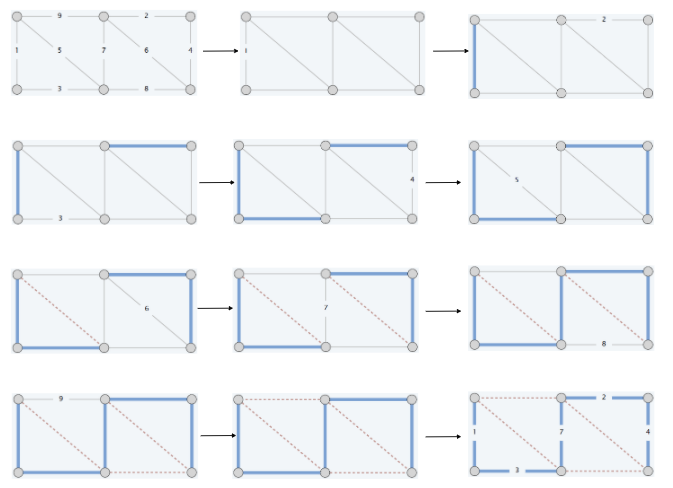
\includegraphics[scale=0.5]{image/kruskal.png}
	\caption{Kruskal算法的执行流程}\label{fig:kruskal}
\end{figure}

\subsection{算法正确性证明}
Kruskal算法每次会向T添加一条最小权重的边,并且不能形成环.
对于一棵树而言, 如果有K个节点, 则必然有K-1条边
我们要证明的问题其实是连续添加的边E(l) l=0,1,2...K-1 是一颗最小生成树MST的子集.

对于基本情况, 如果I = 0, 此时为空集,满足条件;

现在我们假设对 $0 \leq m < K-1$, E(m) 已经满足条件,是$T_1$的子集. 我们来看 E(m+1)的情况,
有E(m+1) = E(m) + {e}, e为算法当前新增的最小权重边.此时分两种情况:

\begin{enumerate}
	\item 如果{e}是$T_1$的子集,那么问题解决;
	\item 如果{e}不是$T_1$的子集, 那么我们要证明 E(m+1) 属于一颗其他的MST子集:

	因为{e}不是$T_1$的边, 所以 $T_1$ + {e} 必然有环C(性质1), 同时 E(m) 属于 $T_1$ ,
	那么在环C上必然有一个{e'} 不属于E(m) (因为如果属于E(m)的化, 那么算法当前选择的{e}会导致一个环, 与性质1违背).
	
	现在我们定义$T_2$ = $T_1$ + {e} - {e'}, 又因为E(m+1) = E(m) + {e} 所以 E(m+1) 属于$T_2$的子集.$T_2$是一颗MST.
	
	因为{e} 和 {e'} 都不属于 E(m), 算法当前选择的是{e} 说明 $weight({e'}) \geq weight({e})$.
	所以我们看$weight(T_2) = weight(T_1) + weight({e}) - weight({e'}) \leq weight(T_1)$ .
	
	这意味着$T_1$是$T_2$的权重upper-bound, 但由于$T_1$已经是MST, 所以必然的$T_2$也是MST. 至此得证.	
\end{enumerate}

\subsection{算法复杂度分析及优化}
\begin{theorem}{}{Kruskal-theorem}
	Kruskal’s algorithm can be implemented to run in $O(m log m)$ time.
\end{theorem}

\begin{enumerate}
	\item Sort edges by cost:$O(m log m)$.
	\item Use union–find data structure to dynamically maintain connected components:$O(m \alpha (n))$.
\end{enumerate}

\begin{remark}
	$\alpha (n)$是反阿克曼函数,阿克曼函数 $A(m,n)$ 增长极快,其反函数几乎是常数。
\end{remark}

下面将简要介绍并查集(union–find data structure)有关内容。
\subsection{并查集}
在计算机科学中,并查集是一种树型的数据结构,用于处理一些不交集(Disjoint Sets)的合并及查询问题。
有一个联合-查找算法(union-find algorithm)定义了两个用于此数据结构的操作:

Find:确定元素属于哪一个子集。它可以被用来确定两个元素是否属于同一子集。

Union:将两个子集合并成同一个集合。

在并查集森林中,每个集合的代表即是集合的根节点。“查找”根据其父节点的引用向根行进直到到底树根。
“联合”将两棵树合并到一起,这通过将一棵树的根连接到另一棵树的根。实现这样操作的一种方法是

\begin{lstlisting}
function MakeSet(x)
     x.parent := x

function Find(x)
     if x.parent == x
        return x
     else
        return Find(x.parent)

function Union(x, y)
     xRoot := Find(x)
     yRoot := Find(y)
     xRoot.parent := yRoot
\end{lstlisting}

这是并查集森林的最基础的表示方法,这个方法不会比链表法好,这是因为创建的树可能会严重不平衡;然而,可以用两种办法优化。

第一种方法,称为“按秩合并”,即总是将更小的树连接至更大的树上。因为影响运行时间的是树的深度,
更小的树添加到更深的树的根上将不会增加秩除非它们的秩相同。在这个算法中,术语“秩”替代了“深度”,因为同时应用了路径压缩时秩将不会与高度相同。

第二个优化,称为“路径压缩”,是一种在执行“查找”时扁平化树结构的方法。关键在于在路径上的每个节点都可以直接连接到根上;
他们都有同样的表示方法。为了达到这样的效果,Find递归地经过树,改变每一个节点的引用到根节点。得到的树将更加扁平。

\chapter{最小生成树其他算法}

\begin{introduction}
	\item red/blue算法
	\item Boruvka算法
\end{introduction}

本章将介绍求解最小生成树的red/blue算法和Boruvka算法。

\section{red/blue算法}

\subsection{基本概念}
下面给出red/blue算法有关内容的定义
\begin{definition}{割(cut)}{cut}
	S$\in$V,S$\neq \emptyset$,点集V被划分成互补的子集S和V/S。
\end{definition}

\begin{definition}{割边集(cutset)}{cutset}
    对于图G的顶点集V的割X、Y,图G的边集E中连接两集合X、Y的所有边的集合叫做这个割的割边集(cutset)。
\end{definition}

\begin{definition}{Red Rule}{Red Rule}
    找到图G中不含红色边的环C,从C中未被染色的边中选出边权最大的边将其染成红色。
\end{definition}

\begin{definition}{Blue Rule}{Blue Rule}
    找到图G中不含蓝色边的割边集D,从D中未被染色的边中选出边权最小的边将其染成蓝色。
\end{definition}

\subsection{算法运行步骤}
\begin{enumerate}
	\item 初始化:对于给定的图G,将所有边标记为未染色。
	\item 在图G中同时运行Red Rule和Blue Rule (可并行运行),直到所有边均被染色为止。
	\item 图G中所有的蓝色边即为图G的最小生成树。
\end{enumerate}

算法具体执行过程如\autoref{fig:redblue}
\begin{figure}[hbt]
	\centering
	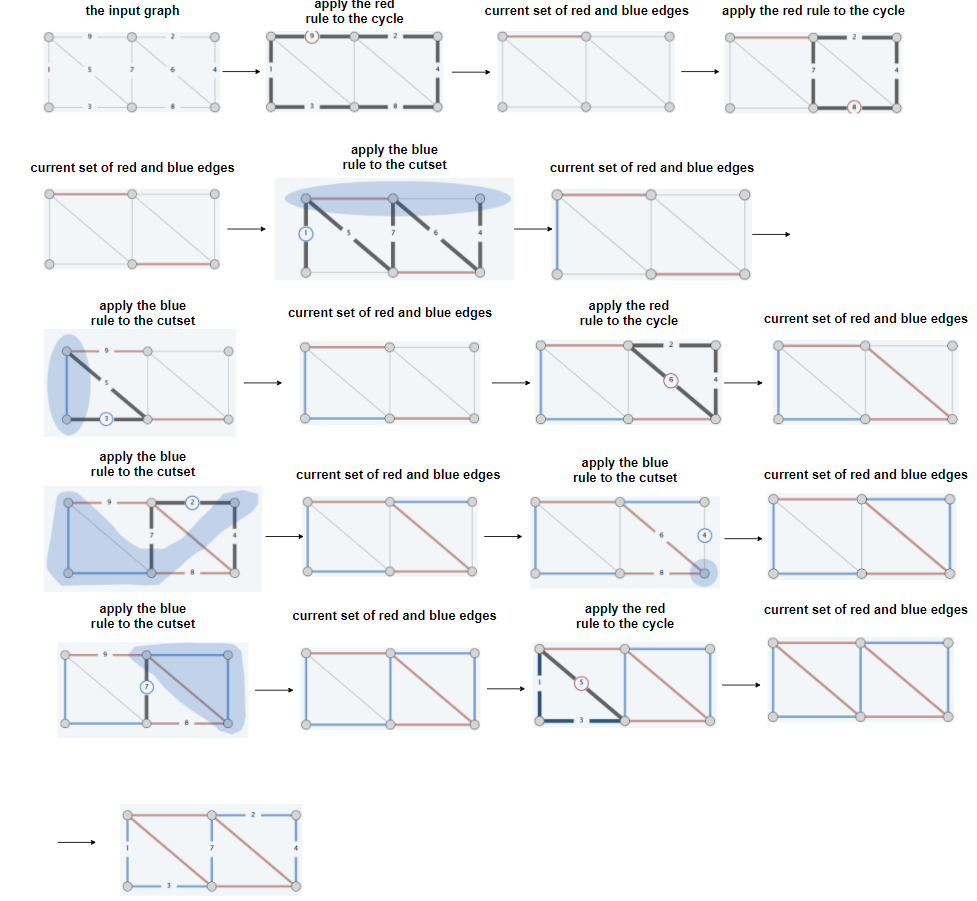
\includegraphics[scale=0.4]{image/redblue.png}
  \caption{red/blue算法执行过程图解}\label{fig:redblue}
\end{figure}

\subsection{算法正确性证明}\label{sec:redblue-proof}
\begin{enumerate}
	\item 最优性:Blue Rule染色所得边为最小边

对于图G中的一个割边集D及D中边权最小的边minEdge,如果在Blue Rule运行过程中被染色的是割边集D的其他边biggerEdge,
则可以在最后得到的MST中将biggerEdge从中删除然后将minEdge加入到MST中,可以得到更小的最小生成树。产生矛盾。所以Blue Rule染色所得边为最小边。
\item 合法性:算法所得所有蓝边为无环连通图

由于Blue Rule可知每次选边都不会成环。下证所得为连通图,假设最后所得所有蓝边构成的图不连通或仍然有点未被蓝边连接。

对于第一种情况,则任选某一蓝边的一个顶点并从该顶点开始的所有能通过蓝边的顶点记为集合X,
S与V/S构成图G的一个割,由Red Rule中所选环C不含红色边可知其割边集不可能全部被染成红色,则说明一定有未染色的边,再应用一次Blue Rule即可增大S的点的个数,
重复上述过程直到S=E;对于第二种情况,由于孤立点必不可能在某个环中,所以连接该点的边一定不会被Red Rule染成红色,所以此时应用一次Blue Rule即可使得该点被蓝边连接。综上,算法所得所有蓝边为连通图
\end{enumerate}

\section{Boruvka算法}
\subsection{算法运行步骤}
\begin{enumerate}
	\item 初始化:对于给定的图G,将所有边标记为未染色;将每个顶点作为一个连通块。
	\item 对于所有蓝边连成的连通块应用Blue Rule并将所有Blue Rule选中的边染成蓝色,直到只有一个连通块。
	\item 最后得到的蓝边连成的连通块即为图G的最小生成树。
\end{enumerate}

算法具体执行过程如\autoref{fig:boruvka}
\begin{figure}[h]
	\centering
	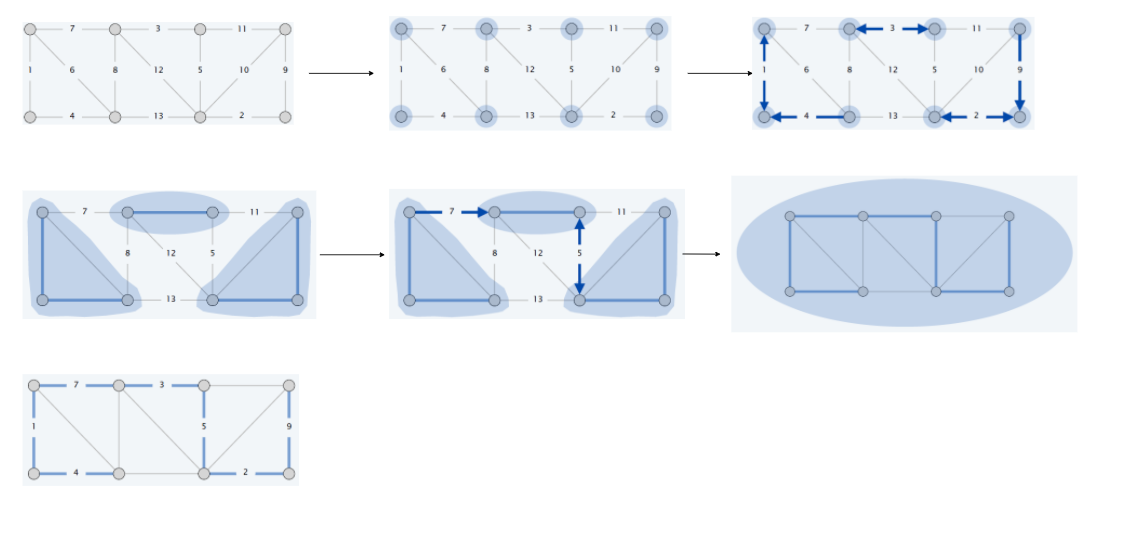
\includegraphics[scale=0.4]{image/boruvka.png}
  \caption{boruvka算法执行过程图解}\label{fig:boruvka}
\end{figure}

算法复杂度分析:每次应用Blue Rule后连通块数量至少减半,每次都要遍历所有边,所以算法串行时间复杂度为O(E$\log V$),并行时间复杂度为O(E)。

\subsection{算法正确性证明}
\begin{enumerate}
	\item 最优性:根据~\ref{sec:redblue-proof}中的证明:Blue Rule染色所得边为最小边。
	\item 合法性:一定不会构成环。如果存在环说明一个点的最小连边有两个,与Blue Rule矛盾。
\end{enumerate}

\input{src/Ln9-NearestPoints.tex}
\input{src/Ln11-LargeIntegerMultiplication.tex}
\input{src/dynamic-programming-1.tex}
\chapter{字符串编辑距离}

\begin{introduction}
	\item 问题引入
	\item 相关概念
	\item 算法思想
\end{introduction}

\section{问题引入}
如何定义两个字符串的距离呢?ocurrance和occrrence有多大的区别呢?下面我们将讨论两个字符串的距离问题。
\section{相关概念}
\begin{definition}{匹配M}{matching}
	字符串X有$x_1$到$x_n$共n个字符,字符串Y有$y_1$到$y_m$共m个字符。X和Y之间存在一个匹配M,其满足:$if (i,j) \in M, (l,k)\in M, i<l iff j<k$。
\end{definition}

%距离代价:

%$\alpha_{xy}$ :两个不同的字符x和y相匹配的代价,则$\alpha_{xy}=0$.

%$\delta$ :每存在一个没有被选择的字符就会多一个$\delta$.

%总距离代价:所有$\delta$ 和 $\alpha$ 的和。

\begin{definition}{距离代价}{penalty}
	$\alpha_{xy}$:两个不同的字符x和y相匹配的代价,则$\alpha_{xy}=0$.
	
	$\delta$:每存在一个没有被选择的字符就会多一个$\delta$.
	
	总距离代价:所有$\delta$ 和 $\alpha$ 的和。
\end{definition}

示例:

\begin{figure}[htb]
	\centering
	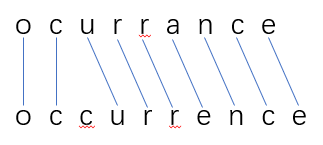
\includegraphics[scale=0.6]{image/connect1.png}
	\caption{字符串匹配}\label{fig:connect1}
\end{figure}
如上图所示,其中的总距离代价为$\alpha_{ae} + \delta$

\section{算法思想}
从后往前推:

bopt (i,j):字符串$x_1,\ldots,x_i$和$y_1,\ldots,y_j$之间的最佳匹配
\begin{equation}
	bopt (m,n)=\begin{cases}
		bopt(m-1,n-1)+\alpha_{x_m y_n} & \text{$x_m$和$y_n$ 相连} \\
		bopt (m-1,n)+\delta            & \text{$x_m$跳过}         \\
		bopt (m,n-1)+\delta            & \text{$y_n$跳过}
	\end{cases}
\end{equation}

从前往后推:

fopt (i,j):字符串$x_i,\ldots,x_m$
和
$y_j,\ldots,y_n$
之间的最佳匹配
\begin{equation}
	fopt (1,1)=\begin{cases}
		fopt(2,2)+\alpha_{x_1 y_1} & \text{$x_1$和$y_1$ 相连} \\
		fopt (2,1)+\delta          & \text{$x_1$跳过}         \\
		fopt (1,2)+\delta          & \text{$y_1$跳过}
	\end{cases}
\end{equation}
初始化:
$bopt (i,0) = \delta_i  $    $bopt (0,i) = \delta_j$

构造图:

\begin{figure}[htb]
	\centering
	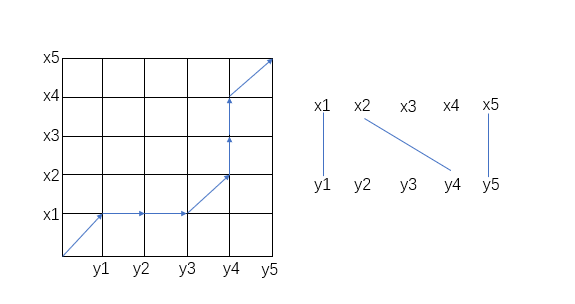
\includegraphics[scale=0.6]{image/connect2.png}
	\caption{构造图}\label{fig:connect2}
\end{figure}
按图构造方法如图所示

\chapter{动态规划之最短路径算法}

\begin{introduction}
	\item Dijkstra算法
	\item Bellman-Ford算法
	%\item 提要3
	%\item 提要4
	%\item 提要5
\end{introduction}


\section{最短路径定义}
给的一个带权重的有向图$G=(V,E)$和权重函数$\omega : E\rightarrow R$,该权重函数将每条边映射到实数值的权重上。图中一条路径$p=<v_0,v_1,...,v_k>$的权重$\omega (p)$是构成该路径的所有边的权重之和:$$\omega (p)=\sum\limits_{i=1}^k\omega (v_{i-1},v_i)$$

定义从结点$u$到结点$v$的最短路径权重


\begin{equation}
\delta(u,v) = \begin{cases}
min( \omega (p) : u\stackrel{p}{\longrightarrow} v )  & uv\text{连通} \notag\\
+\infty   &  uv\text{不连通}

\end{cases}
\end{equation}


从结点$u$到结点$v$的最短路径则定义为任何一条权重为$\omega (p)=\delta(u,v)$的从结点$u$到结点$v$的路径$p$

对于每个节点,我们定义两个属性。v.d用来记录源节点s到节点v的最短路径权重上界。v.f用来记录节点v的前驱节点。

定义初始化和松弛两个操作。

\begin{lstlisting}[caption=初始化和松弛伪代码]
INITIALIZE-SINGLE-SOURCE(G,s)
for each vertex v in G.V
    v.d=$\infty$
    v.f=NULL
s.d=0

RELAX(u,v)
if v.d>u.d+(u,v)
    v.d=u.d+(u,v)
    v.f=u
\end{lstlisting}

\section{Dijkstra算法}
Dijkstra算法解决的是一般情况下的单源最短路径问题,边的权重要求为非负值。

Dijkstra算法在运行过程中关键是维护一个结点的集合$S$。从源节点$s$到该集合中的每个结点之间的最短路径已经找到。该算法重复
从结点集$V-S$中选择离源节点最近的结点$u$加入到集合$S$中。然后重新计算源节点到其余各点的距离。如此以往,直到所有点都加入到集合$S$中。

\begin{lstlisting}[caption=Dijkstra算法伪代码]
DIJKSTRA(G,S)
INITIALIZE-SINGLE-SOURCE(G,s)
S=NULL
Q=G.V
while Q!=NULL
	u=EXTRACT-MIN(Q)
	S=S+u
	for each vertex v in G.Adj[u]
		 RELAX(u,v)
\end{lstlisting}

算法运行过程如下:

\begin{figure}
\centering
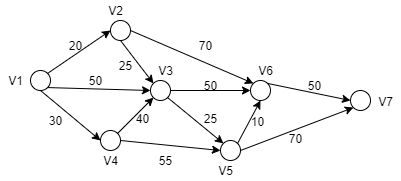
\includegraphics[width=10cm,height=5cm]{image/dijkstra1.png}
\caption{一个带权有向图}
\end{figure}
\begin{figure}
\centering
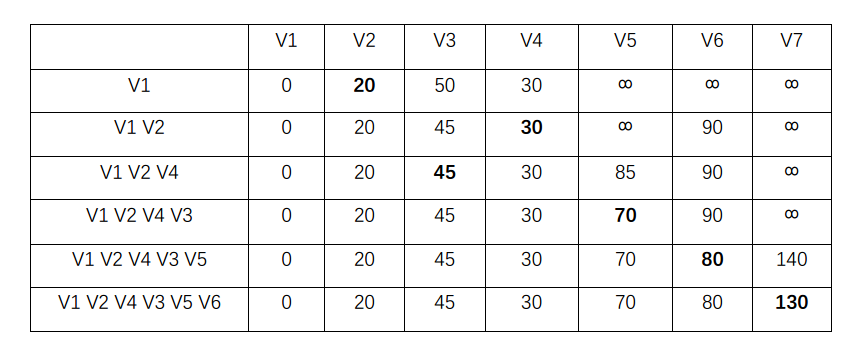
\includegraphics[width=10cm,height=5cm]{image/dijkstra2.png}
\caption{对应Dijkstar算法执行过程表格}
\end{figure}

表的左侧是当前的集合。表中每一行的数字为源点通过集合中的点到各点的当前最短路径距离。在表中加粗的数字对应的节点为该轮中将被加入到集合$S$中节点。

\subsection{时间复杂度}
算法第1行初始化操作所需时间为$\Theta(V)$,第4行循环一共执|V|次,其中第5行操作所需时间为$O(V)$,第7行的for循环在整个算法执行期间一共执行|E|次,故Dijkstra算法的总运行时间为$O(V^2+E)=O(V^2)$

\subsection{正确性证明}
Dijkstra算法使用贪心的策略,每次选择”最近“的节点加入到集合中。下面通过对已经访问的节点数学归纳法证明其正确性。

\begin{enumerate}
\item 当只有两个节点的时候,显然成立。

\item 假设n-1个结点时。现在我们选择一条边(v,u),其中节点u是未访问结点中具有最小的u.d的节点,并且$u.d=v.d+\omega(v,u)$。u.d必定是源点到所有未访问中最短路径长度。因为假如有一条更短的路径,假设k是该路径上第一个未访问的节点,这与假设$k.d>u.d$矛盾,所以u.d必定是源点到所有未访问节点中最短路径长度。类似,如果在没有使用未访问节点情况下存在一条到节点u的更短路径,并且如果该路径上最后一个节点是k,则我们有$u.d=k.d+\omega(k,u)$,与前提矛盾。其余未访问节点同理。
\end{enumerate}

综上所述,Dijkstra算法正确。

\section{Bellman-Ford算法}
Bellman-Ford算法解决的是一般情况下的单源最短路径问题,边的权重可以为负值。

由分析可知,s到t的最短路一定是一个简单路径。并且最短路径的边数小于等于n-1(n为节点数)。我们记opt(v,k)为从v到t,边数小于等于k的最短路径。考虑两种情况,一种是最短路径边数小于等于k-1,一种是边数等于k的。
则有
$$opt(v,k)=min(opt(v,k-1),\min \limits_{(v,w)\in E}(opt(w,k-1)+c(v,w)))$$
其中w是与v直接相连的点。

同理还可以记opt(t,k)为从v到t,边数小于等于k的最短路径。则有
$$opt(t,k)=min(opt(t,k-1),\min \limits_{(w,t)\in E}(opt(w,k-1)+c(w,t)))$$

\begin{lstlisting}[caption=Bellman-Ford算法算法伪代码]
BELLMAN-FORD(G,s)

INITIALIZE-SINGLE-SOURCE(G,s)
for i=1 to |G.V|-1
	for each edge(u,v) in G.E
 		RELAX(u,v)
for each edge(u,v) in G.E
	if v.d>u.d+(u,v)
		return FALSE
return TRUE

\end{lstlisting}

\subsection{时间复杂度}
算法第1行初始化操作所需时间为$\Theta (V)$,第2到4行循环的运行时间为$\Theta (E)$,且一共要进行|V|-1次循环,第5到7行的for循环所需时间为$O(E)$,Bellman-Ford算法的总运行时间为$O(VE)$。

\subsection{正确性证明}
若某节点和源点不连通,初始化时,除了源点的距离为0外,其他节点的初始化为无穷大。如果不连通,则该节点所在的连通图的任一条边都不会导致更新。

若节点x点与源点连通。每个点都存在自己的最短路,为$(e_0,e_1,e_2,...,e_k)$。显然,源点只要经过|V|-1条边就可到达任一点。

现只需证明,对节点v,每次松弛操作,至少有一条最短边$e_i$的距离被找到,除非已经到达v点。

对于第一次松弛,必定更新和源点s相连的所有出边。由于源点s初始距离是0,和其相连的节点初始距离都是无穷大。而这些相连的出边中,必有一条是节点v的最短路上起始的一条边。则设有节点k,这个节点是节点v最短路上的一共点,由于下一次松弛将更新与k相连的所有点,必能找到下一个点,且也是节点v的最短路径上的一个点。则通过多次松弛可以找出最短路。

综上所述,Bellman-Ford算法正确。

\input{src/LN18-DP-ZeroOneKnapsack.tex}
\input{src/Ln19-DP-ContextFreeGrammar.tex}
\input{src/Network-flows.tex}
\chapter{网络流应用之图像分割}

{\centering 本章简单介绍网络流在图像分割上的应用。}

\begin{definition}{背景知识}{}
	图像是可以看作由一个个像素组成的巨大图, 将像素一一用边连接起来, 则这些像素点会成为这个巨大图网络的顶点.
	一个图由前景和背景组成, 假设顶点上的值用 $a_i$ 表示, $ 0 \leq a_i \leq 1 $,  $a_i$ 趋近于 0 表示 $a_i$ 为图的背景, $a_i$ 趋近于 1 表示 $a_i$ 为图的前景, 并且设所有属于前景的顶点 $a_i$ 构成集合 A, 所有属于背景的顶点 $a_j$ 构成集合 B.
	假设边上的值用 $w_{ij}$ 表示, $w_{ij}$ 设为边的惩罚值, $w_{ij}$ 趋向于 0 表示“分离” (即 $w_{ij}$ 连接的两个点分别属于前景和背景), $w_{ij}$ 趋向于 1 表示“在一起” (即 $w_{ij}$ 连接的两个点都属于前景或者背景)
	设总的惩罚值为 $ A = \min\left(\sum_{i \epsilon B}a_i +  \sum_{i \epsilon A}(1 - a_j) + \sum_{i \epsilon A, j \epsilon B}w_{ij} \right) $
\end{definition}


\section{问题实例}
\subsection{问题描述}
\begin{itemize}
	\item 对于下面这个图,利用网络流求解该图前景和背景的最大可能
\end{itemize}

\begin{figure}[htb]
	\centering
	\includegraphics[scale=0.8]{image/Image-segmentation2.png}
	\caption{图片前景背景识别}\label{fig:image-seg-1}
\end{figure}

\subsection{思路描述}
\begin{itemize}
	\item 图形切割算法通过向图 G (V,E) 添加 S 点和 T 点,将图中所有的顶点,与 S 和 T 建立边,
	      如果一个点与 S 相连,则对应边的权值为该点的值 $a_i$, 如果一个点与 T 相连,则对应边的权值为1减去该点的值 $ 1 - a_j $。
	      可以得到下面这个图:
\end{itemize}

\begin{figure}[htb]
	\centering
	\includegraphics[height=4.5cm]{image/Image-segmentation3.png}
	\caption{图片前景背景识别}\label{fig:image-seg-2}
\end{figure}

\begin{itemize}
	\item   根据最大流最小割, 可以得到得到二分图的最大匹配, 可以得到集合A和B, 保证总的惩罚值 $ A = \min\left(\sum_{i \epsilon B}a_i +  \sum_{i \epsilon A}(1 - a_j) + \sum_{i \epsilon A, j \epsilon B}w_{ij} \right) $ 最小,
	      最小为 $(0.2 + 0.1) + (1 - 0.9) + (1 - 0.8) + 0.3 + 0.3 = 1.2 $, 而 A 和 B 分别对应图的前景和背景。
\end{itemize}

\section{问题扩展}
\begin{itemize}
	\item 假如一个图的前景不是一个整体,
	      而是有两个分开的部分,比如两只在两个不同位置的猫在一个图中。
	      这样一个算法能否将图像上的前景和背景分开?
\end{itemize}

\begin{figure}[htb]
	\centering
	\includegraphics[scale=0.6]{image/Image-segmentation1.png}
	\caption{图片前景背景识别}\label{fig:image-seg-3}
\end{figure}

\input{src/Ln26-P-NP.tex}
\chapter{规约证明: 顶点覆盖  独立集}

\begin{introduction}
	\item 顶点覆盖
	\item 独立集
	\item 顶点覆盖和独立集的相互规约
\end{introduction}


\section{顶点覆盖}

\begin{theorem}{xxx定理}{label-for-this-theorem}
	这是一个定理。
\end{theorem}


\begin{definition}{定义}
	对于一个图 G = (V, E),V是图中所有节点的集合,E是图中所有边的集合,那么图G中的一个顶点覆盖是点集 V 的一个子集 S,S $ \subseteq $ V ,使得 G 中的每一条边的两个端点至少有一个在 S 中
\end{definition}

\begin{definition}{形式化定义}
    给定图 G = (V,E),图节点集合V,图边集合E,图的一个顶点覆盖 S ,有S $ \subseteq $ V,并且 ∀ (u, v) $ \in $ E (u, v $ \in $ V), u $ \in $ S 或者 v $ \in $ S
\end{definition}

\begin{example}
    如下图所示
	\begin{figure}[hbt]
        \centering
        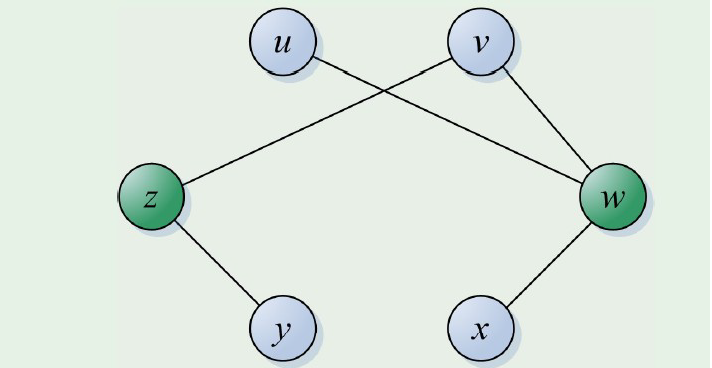
\includegraphics{image/Proof-of-Statute1.png}
        \caption{图中节点z, w组成的集合是一个顶点覆盖。}\label{fig:example}
    \end{figure}
\end{example}

\begin{definition}{最小顶点覆盖}
    最小顶点覆盖是图的一个顶点覆盖,并且其中的节点数最少。其形式化定义为:对于所有的顶点覆盖组成的集合 S = {$ S_1 $, $ S_2 $, ..., $ S_n $},最小顶点覆盖 $ S_m $,有 $ S_m \in $ S,∀ $ S_i \in $ S (i ≠ m), |$ S_i $| ≥ |$ S_m $|
\end{definition}


\section{独立集}

\begin{definition}{定义}
    图的一个顶点子集称为独立集,如果该子集中的任意两个项点在图中不相邻,也即没有边连接这两个点。
\end{definition}

\begin{definition}{形式化定义}
    给定图 G = (V,E),图节点集合 V,图边集合 E,图的一个独立集 S,S $\subseteq$ V,有 ∀u, v $\in$ S,(u,v) $\notin$ E
\end{definition}

\begin{example}
    如下图所示
	\begin{figure}[hbt]
        \centering
        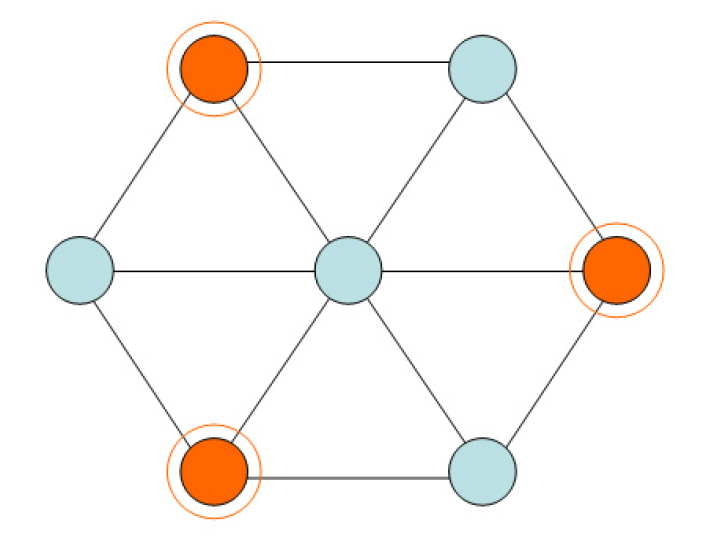
\includegraphics{image/Proof-of-Statute2.png}
        \caption{图中三个橙色的点构成图的一个独立集}\label{fig:example}
    \end{figure}
\end{example}

\begin{definition}{最大独立集}
    最大独立集是图的一个独立集,并且其中的节点数最多。其形式化定义为:对于图 G = (V,E) 所有的独立集组成的集合 S = {$ S_1 $, $ S_2 $, ..., $ S_n $},最大独立集 $ S_m $,有 $ S_m \in $ S,∀ $ S_i \in $ S (i ≠ m), |$ S_i $| $ \leq $ |$ S_m $|
\end{definition}


\section{顶点覆盖问题与独立集问题的相互规约}

\begin{theorem}{定理一}
    一个有n 个结点的图存在一个大小为k 的独立集,当且仅当这个图存在一个大小为n-k 的定点覆盖
\end{theorem}

\begin{proof}
    \begin{itemize}
        \item 当S是G的顶点覆盖时,V−S是G的独立集。当S是G的顶点覆盖时,V−S是G的独立集。也就是说对于(u,v) $\in$ E, u $\in$ S或者 v $\in$ S 或者 u, v $\in$ S,那么当只有 u $\in$ S时,可以将 v 放到独立集 S′ 中,对于 v 同理,如果 u, v $\in$ S,那么对于(u,v) 这条边的两个端点都不可以放入S′中。由于(u,v) 任意,根据上面的方法,u,v必然在S、S′中的一个集合中,因此 S $\cup$ S′= V,并且此时形成的独立集中任意两个点u′, v′, (u′, v′) ∉ E,否则在上面描述的方法中,u′, v′不可能全部放入独立集S′中。
        \item 当S是G的独立集时,V−S 是G的顶点覆盖。如果一个图G= (V , E) 有n个节点,它有一个k个节点的独立集S,则对于G中的任意一条边,其最多有一个端点在S中,也就是说对于(u,v) $\in$ E, u $\notin$ S或者 v $\notin$ S 或者 u, v $\notin$ S,那么当 u $\notin$ S时,可以将 u 放到顶点覆盖S′中,对于v同理,如果u,v∉S,那么可以将u,v都放入到顶点覆盖S′ 中。由于(u,v) 任意,根据上面的方法,u,v必然在S、S′中的一个集合中,因此 S $\cup$ S′= V,并且此时对于 ∀(u,v) $\in$ E,u $\in$ S′ 或者 v $\in$ S′ 或者 u, v $\in$ S′,否则根据上面描述的方法,必然没有遍历完所有的边。
    \end{itemize} 
\end{proof}


\begin{theorem}{定理二}
    一个有n 个结点的图存在一个最大独立集,当且仅当这个图存在一个最小定点覆盖
\end{theorem}

\begin{proof}
    对于一个图G= (V, E),其可能存在多个独立集,它们构成一个独立集集合S = {S1, S2, ..., Sn},我们可以找出其中结点数最多的一个独立集Sm,有k个节点,这就是这个图的最大独立集,那么由定理1,这个图就会有一个n-k 的一个顶点覆盖,这个顶点覆盖是图的最小顶点覆盖,可以使用反证法结合定理1 证明其正确性。
    同理,反过来我们可以找到图的一个大小为k 的最小顶点覆盖,那么根据定理1,可以得到一个大小为n-k 的独立集,这个独立集就是图的最大独立集,同样可以使用反证法结合定理1 证明其正确性。
\end{proof}
\chapter{近似算法}

\begin{introduction}
	\item 近似算法介绍
	\item 顶点覆盖
	\item 任务调度
	\item 最小带权覆盖
	\item MAX-K-SAT
\end{introduction}

本章讲述了NPC问题的一些近似算法及其质量分析。

\section{近似算法介绍}

\subsection{引入与定义}

求解NPC问题的思路通常包括:
\begin{enumerate}
	\item 设计通用的指数级时间复杂度算法
	\item 针对特例设计多项式时间复杂度算法
	\item 根据问题特点设计启发式算法,或借用元启发式算法的框架求解(如蚁群、遗传、退火等算法)
	\item 设计近似算法
\end{enumerate}
其中设计近似算法时便要求时间复杂度是多项式级,得到的解可以保证与最优解比差别有限,具体定义如下。

\begin{definition}{近似算法}{approximation-algorithm:15Ln-ApproximationAlgorithm}
	对一个最小最优问题(最大最优则变为大于号)有多项式级时间复杂度,并对任意实例均有$ALG\leqslant \alpha \cdot OPT$,其中$\alpha$为一个常数,则称该算法为此问题的近似算法。(ALG为该算法结果的质量,OPT为最优解的质量)
\end{definition}

\subsection{近似算法常用证明方法}

\begin{figure}[htb]
	\centering
	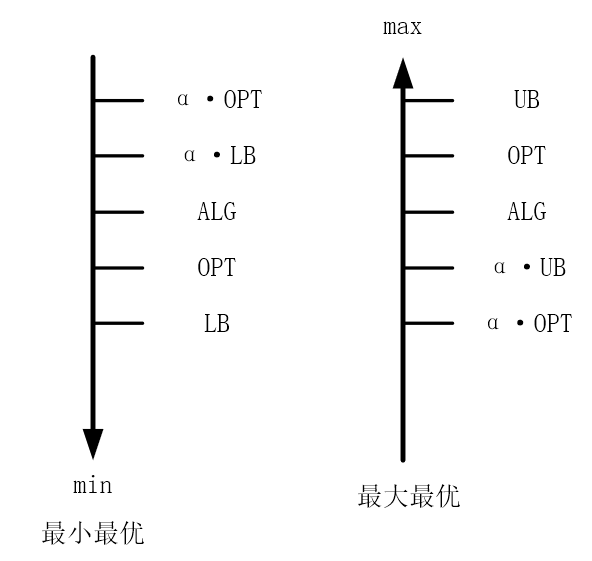
\includegraphics[scale=0.3]{image/Ln15-ApproximationAlgorithm1.png}
	\caption{近似算法证明思路} \label{proof:Ln15-ApproximationAlgorithm}
\end{figure}

\subsubsection{最小最优证明}
一般利用\autoref{proof:Ln15-ApproximationAlgorithm}的证明思路,首先找到OPT下界LB,证明$OPT\geqslant LB$,再想办法证明$ALG\leqslant \alpha \cdot LB$,从而得到$ALG\leqslant \alpha \cdot OPT$,即可证明该近似算法的正确性。
\subsubsection{最大最优证明}
同样利用\autoref{proof:Ln15-ApproximationAlgorithm}的证明思路,首先找到OPT上界UB,证明$OPT\leqslant UB$,再想办法证明$ALG\geqslant \alpha \cdot UB$,从而得到$ALG\geqslant \alpha \cdot OPT$,即可证明该近似算法的正确性。



\section{顶点覆盖}

本节将介绍一个顶点覆盖的近似算法。

\subsection{问题描述}

\begin{definition}{顶点覆盖问题}{vertex-cover:15Ln-ApproximationAlgorithm}
	对于给定的图$(V,E)$,找到一个点集$S\subset V$,使得该图所有边都至少有一个端点在点集S中。
\end{definition}

\subsection{算法描述}

算法步骤如下:
\begin{enumerate}
	\item 找到极大匹配M,相关定义如下:
	\begin{definition}{匹配}{matching:15Ln-ApproximationAlgorithm}
		给定一个图G,在G的一个子图M中,任意两边都没有相同的端点,且每个点都有边相连。
	\end{definition}
	\begin{definition}{极大匹配}{maximal-matching:15Ln-ApproximationAlgorithm}
		一个匹配无法再增加任何点和边,则称之为极大匹配。
	\end{definition}
	\item 输出M中的所有点作为解的点集S
\end{enumerate}

\subsection{正确性证明}

\begin{proof}
该算法始终有$ALG\leqslant 2\cdot OPT$,在该问题中OTP即为最优解点的数量,ALG即为算法求解的点的数量。
\end{proof}
\begin{enumerate}
	\item 证明$OPT\geqslant |M|$(其中|M|为极大匹配的边数):对于M中任意一条边,其必定至少有一点在OPT中,否则这条边就未被覆盖,与顶点覆盖的要求矛盾。故$OPT\geqslant |M|$
	\item 证明$ALG=2\cdot |M|$:极大匹配中任意一点度为1,故点的数量即为边的数量的两倍,得证$ALG=2\cdot |M|$。
	\item 根据上述证明可以得到$2\cdot OPT\geqslant 2\cdot|M|=ALG$,得证$ALG\leqslant 2\cdot OPT$
\end{enumerate}
	
\section{任务调度}

\subsection{问题描述}
定义任务$T$为集合$\{t_1,t_2,\ldots,t_n\}$,有$m$台机器$\{M_1,M_2,\ldots,M_m\}$,而一任务调度即将任务$T$中的所有任务分配给这$m$台机器,假设对第$i$台机器,设其被分配的任务为集合$A(i),i\in [1,m]$,则其执行任务的总时间可定义为
\begin{equation*}
	T_i=\sum_{j\in A(i)} t_j
\end{equation*}
所有机器并行执行任务,则完成所有任务的时间$T$可表示为
\begin{equation*}
	T=\max_{i=1}^{m} T_i
\end{equation*}
要求寻找一个算法,使得$T$尽可能的小,设实际最优解为$T_0$

该问题为$NP-hard$问题,所以无法在多项式找出最优解,以下给出的均为近似算法,并讨论解与最优解的关系。

\begin{example}
	假设有6个任务,其所需执行时间依次为2,3,4,6,2,2,有三台机器,则其最优解$T_0=7$。
\end{example}

\subsection{贪心算法一[在线算法]}
该问题最直接的思路就是贪心算法,将依次取$t_1,t_2,\ldots,t_n$,让$m$台机器执行,每次挑选的机器的$T_i$都是最小的,即每次$t_i$都加入到当前负载$T_k$最小的机器,设该算法给出的近似解为$T_1^*$

算法的伪代码如下

\begin{algorithm}
	\DontPrintSemicolon{}
	\KwResult{the minimum $T_1^*$}
	\Begin{
		Start with no tasks assigned\\
		Set $T_i=0$ and $A(i)=\{\}$ for all machines $M_i$
		\ForEach{$j \in [1,n]$}{
			Let $M_i$ be a machine which $T_i$ the minimum at present\\
			Aissign task j to machine $M_i$\\
			Set $A(j)=A(i)\cup \{j\}$\\
			Set $T_j=T_i+t_j$
		}
	}
	\caption{Greedy-Algorithm1}\label{greedy1-algo}
\end{algorithm}

该算法在所给出的例子中运行的结果如下图所示,这里给出的近似解为$T_1^*=6+2=8$
\begin{figure}[hbt]
	\centering
	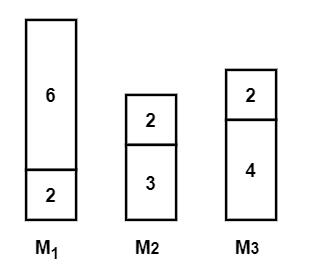
\includegraphics{image/greedy1-result.jpg}
	\caption{贪心算法一的结果}\label{fig:greedy1-result}
\end{figure}

实际上我们可以证明,$T_1^*$和$T_0$有如下关系:
\begin{equation*}
	T_1^*\leq 2T_0
\end{equation*}

证明首先需要用到两个显而易见的定理。
\begin{theorem}{}{label-for-the1}
	最优解$T_0$不可能比所有任务在所有机器执行的平均时间还小,即
	\begin{equation*}
		T_0\geq \frac{\sum_j t_j}{m}
	\end{equation*}
\end{theorem}

\begin{theorem}{}{label-for-the2}
	最优解$T_0$不可能比任务时间最长的那个任务的时间小,即
	\begin{equation*}
		T_0\geq \max_j t_j
	\end{equation*}
	因此$T_0$会大于等于任一$t_i$。
\end{theorem}

进一步假设由该贪婪算法所得到的$T_1^*$由第i台机器产生,如下图所示
\begin{figure}[hbt]
	\centering
	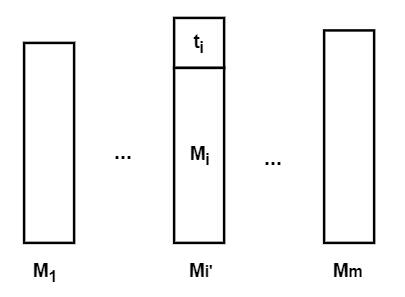
\includegraphics{image/greedy1-proof.jpg}
	\caption{贪心算法一近似比的证明}\label{fig:greedy1-proof}
\end{figure}

\begin{proof}
	由定理2可知,最上面的那个任务$t_i$的执行时间不会比$T_0$更大,即
	\begin{equation*}
		t_i \leq \max_j t_j \leq T_0
	\end{equation*}
	而$M_i$是所执行的剩下任务的总时间,根据贪婪算法的执行的策略,会导致在使$M_i$执行最上面的那个任务之前,剩下的任务的时间之和是最小的,由定理1可知,该部分时间和不会超过$T_0$,即
	\begin{equation*}
		M_i \leq AVG \leq T_0
	\end{equation*}
	因此,$T_1^*\leq 2T_0$成立。
\end{proof}

\subsection{贪心算法二[先排序再贪心]}
针对贪心算法一,一个很自然的改进措施,将所有任务按照从大到小的时间进行排序,然后再执行贪心算法一。

算法的伪代码如下

\begin{algorithm}
	\DontPrintSemicolon{}
	\KwResult{the minimum $T_2^*$}
	\Begin{
		Start with no tasks assigned\\
		Sort tasks in decreasing order of processing time $t_j$ \\
		Assume that $t_1 \geq t_2 \geq \ldots \geq t_n$
		Set $T_i=0$ and $A(i)=\{\}$ for all machines $M_i$
		\ForEach{$j \in [1,n]$}{
			Let $M_i$ be a machine which $T_i$ the minimum at present\\
			Aissign task j to machine $M_i$\\
			Set $A(j)=A(i)\cup \{j\}$\\
			Set $T_j=T_i+t_j$
		}
	}
	\caption{Greedy-Algorithm2}\label{greedy2-algo}
\end{algorithm}

该算法在所给出的例子中运行的结果如下图所示,这里给出的近似解为$T_2^*=3+2+2=7$
\begin{figure}[hbt]
	\centering
	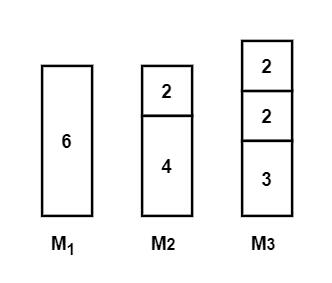
\includegraphics{image/greedy2-result.jpg}
	\caption{贪心算法二的结果}\label{fig:greedy2-result}
\end{figure}

实际上我们可以证明,$T_2^*$和$T_0$有如下关系:
\begin{equation*}
	T_1^*\leq \frac{3}{2} T_0
\end{equation*}

进一步假设由该贪婪算法所得到的$T_2^*$由第i台机器产生,如下图所示
\begin{figure}[hbt]
	\centering
	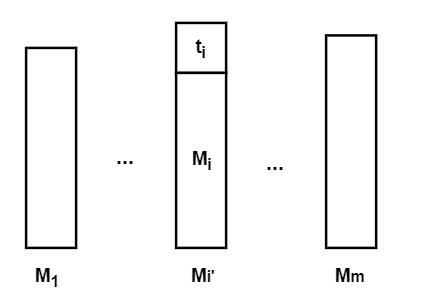
\includegraphics{image/greedy2-proof.jpg}
	\caption{贪心算法二近似比的证明}\label{fig:greedy2-proof}
\end{figure}

\begin{proof}
	首先,如果任务数$n$小于等于机器数$m$,那么显然有$T_2^*=T_0$,结论成立。

	如果任务数$n$大于机器数$m$,则有$T_0 \geq 2t_{m+1}$,因为一开始第$1$到第$m$个任务会被依次放在第$1$到第$m$台机器上,而第$m+1$个任务必然会放在这几个任务之后执行,而由于任务已经按降序排序,故第$m+1$个任务放好之后,必然会大于$2t_{m+1}$,而它必然小于等于$T_0$,即$T_0 \geq 2t_{m+1}$,则有
	\begin{equation*}
		t_{m+1} \leq \frac{1}{2}T_0
	\end{equation*}
	
	在图中,最上面的那个任务$t_i$的执行时间不会比$t_{m+1}$更大(因为序号在m+1后面),即
	\begin{equation*}
		t_i \leq t_{m+1} \leq \frac{1}{2}T_0
	\end{equation*}
	而$M_i$是所执行的剩下任务的总时间,根据贪婪算法的执行的策略,会导致在使$M_i$执行最上面的那个任务之前,剩下的任务的时间之和是最小的,由定理1可知,该部分时间和不会超过$T_0$,即
	\begin{equation*}
		M_i \leq AVG \leq T_0
	\end{equation*}
	因此,$T_2^*\leq \frac{3}{2}T_0$成立。

	综上所述,$T_2^*\leq \frac{3}{2}T_0$成立。
\end{proof}

\subsection{补充}
实际上,对于算法二而言,$\frac{3}{2}$并非下确界,实际上的下确界为
\begin{equation*}
	T_2^*\leq \frac{4}{3} T_0
\end{equation*}

此处下确界的含义是,不可能再找到一个比它更小的正数满足上式。

进一步假设由该贪婪算法所得到的$T_2^*$由第i台机器产生,如下图所示
\begin{figure}[hbt]
	\centering
	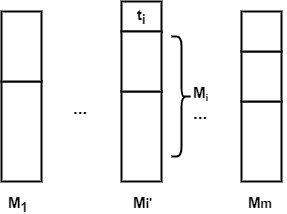
\includegraphics{image/greedy2-proof-4-3.jpg}
	\caption{贪心算法二近似比的证明}\label{fig:greedy2-proof-4-3}
\end{figure}

\begin{proof}
	首先,如果任务数$n$小于等于机器数$m$,那么显然有$T_2^*=T_0$,结论成立。

	然后,如果任务数$n$与机器数$m$的关系满足$n>2m$时,则有$T_0 \geq 3t_{2m+1}$,对于前$2m+1$个任务,由鸽笼原理,必有一个机器分到3个任务,而由于任务已经按降序排序,故第$2m+1$个任务放好之后,这个机器上的3个任务和必然会大于$3t_{2m+1}$,而它必然小于等于$T_0$,即$T_0 \geq 3t_{2m+1}$,则有
	\begin{equation*}
		t_{2m+1} \leq \frac{1}{3}T_0
	\end{equation*}
	
	在图中,最上面的那个任务$t_i$的执行时间不会比$t_{2m+1}$更大(因为序号在2m+1后面),即
	\begin{equation*}
		t_i \leq t_{2m+1} \leq \frac{1}{3}T_0
	\end{equation*}
	而$M_i$是所执行的剩下任务的总时间,根据贪婪算法的执行的策略,会导致在使$M_i$执行最上面的那个任务之前,剩下的任务的时间之和是最小的,由定理1可知,该部分时间和不会超过$T_0$,即
	\begin{equation*}
		M_i \leq AVG \leq T_0
	\end{equation*}
	因此,$T_2^*\leq \frac{4}{3}T_0$成立。

	最后,当$m<n \leq 2m$时,也不能得到$T_0$,只能得到$\frac{4}{3}T_0$,此部分证明复杂。

	综上所述,$T_2^*\leq \frac{4}{3}T_0$成立。
\end{proof}

\begin{example}
	假设有$2m+1$个任务,执行时间分别为$m$到$2m$和$m+1$到$2m$,求解贪心算法二的近似比。
\end{example}
该问题的特殊性使得其最优解可以凭直觉得到为$3m+2$,调度策略如下图所示。
\begin{figure}[hbt]
	\centering
	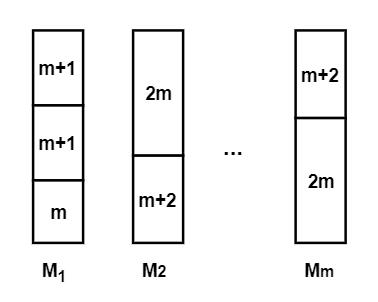
\includegraphics{image/example-problem-opt-solve.jpg}
	\caption{最优解调度}\label{fig:example-problem-opt-solve}
\end{figure}

而利用贪婪算法二得出的近似解$T_2^*$则为$4m+1$,证明如下。
\begin{proof}
	贪心算法二调度策略如下表所示。
	% Please add the following required packages to your document preamble:
	% \usepackage{multirow}
	\begin{table}[]
	\begin{tabular}{cccccccc}
	\hline
	$M_1$					&	$M_2$					&	$M_3$					&	$M_4$					&	...											&	$M_{m-1}$			&	$M_m$				&	m的奇偶性	\\ \hline
	\multirow{2}{*}{$2m$}	&	\multirow{2}{*}{$2m$}	&	\multirow{2}{*}{$2m-1$}	&	\multirow{2}{*}{$2m-1$}	&	\multicolumn{1}{c|}{\multirow{2}{*}{...}}	&	$2m-\frac{m}{2}+1$	&	$2m-\frac{m}{2}+1$	&	偶数m		\\ \cline{6-8} 
							&							&							&							&	\multicolumn{1}{c|}{}						&	$2m-\frac{m+1}{2}+2$&	$2m-\frac{m+1}{2}+1$&	奇数m		\\ \hline
	\multirow{2}{*}{$m+1$}	&	\multirow{2}{*}{$m+1$}	&	\multirow{2}{*}{$m+2$}	&	\multirow{2}{*}{$m+2$}	&	\multicolumn{1}{c|}{\multirow{2}{*}{...}}	&	$2m-\frac{m}{2}$	&	$2m-\frac{m}{2}$	&	偶数m		\\ \cline{6-8} 
							&							&							&							&	\multicolumn{1}{c|}{}						&	$2m-\frac{m+1}{2}$	&	$2m-\frac{m+1}{2}+1$&	奇数m		\\ \hline
	$m$						&							&							&							&												&						&						&				\\ \hline
	4m+1					&	3m+1					&	3m+1					&	3m+1					&	...											&	3m+1				&	3m+1				&
	\end{tabular}
	\end{table}
	
	贪心算法二的调度顺序为从第一排从左到右,第二排从右到左,第三排剩一个m,由表可以得到最大时间为$4m+1$。
\end{proof}

因此贪心算法的近似比为$\lim_{m\to \infty}\frac{4m+1}{3m+2}=\frac{4}{3}$

更一般的,对于算法解$ALG$和最优解$OPT$,有$\frac{ALG}{OPT} \leq \frac{4}{3}-\frac{1}{3m}$。



\section{最小带权覆盖}

本节将介绍一个最小带权覆盖的近似算法。

\subsection{问题描述}

\begin{definition}{最小带权覆盖问题}{weighted-vertex-cover:15Ln-ApproximationAlgorithm}
	对于给定的图$(V,E)$,各个点有权重w,找到一个点集$S\subset V$,使得该图所有边都至少有一个端点在点集S中,且S中所有点的权重之和比所有可行的解都小。
\end{definition}

\subsection{算法描述}

算法步骤如下:
\begin{enumerate}
	\item 将原问题建模为线性规划问题:
	原问题是$\forall e=(u,v)\epsilon E$,有$v\epsilon S$或$u\epsilon S$,求$\min \sum\limits_{v\epsilon G} x_vw_v$其中
	\[
		x_v = \begin{cases}
			0 & v\notin S \\
			1 & v\epsilon S
		\end{cases}
	\]\\
	将其转化为线性规划问题,可变为:
	\[
		\begin{cases}
			x_v^*+x_u^*\geqslant 1 			   &\forall e=(u,v)\epsilon E\\
			x_v^*\geqslant 0	   			   &\forall v\epsilon G, x_v\epsilon [0,1]\\
			\min \sum\limits_{v\epsilon G} x_v^*w_v
		\end{cases}
	\]
	\item 使用线性规划求解器求解,再将得到的解转化为原问题的解:
	\[
		x_v=\begin{cases}
			0 &x_v^*<0.5\\
			1 &x_v^*\geqslant 0.5
		\end{cases}
	\]
\end{enumerate}

\subsection{正确性证明}

\begin{proof}
	该算法得到的解是一个顶点覆盖
\end{proof}
	因为$\forall e=(u,v)\epsilon E,x_v^*+x_u^*\geqslant 1$,故$x_v^*\geqslant 0.5$或$x_u^*\geqslant 0.5$,故$x_v$和$x_u$至少有一个为1,即至少有一点覆盖该边e。得证该算法得到的解是一个顶点覆盖。
\begin{proof}
	$ALG\leqslant 2\cdot OPT$
\end{proof}
	$OPT\geqslant \sum\limits_{v\epsilon G} x_v^*w_v^*$,而又有$x_v\leqslant 2\cdot x_v^*$,故有
	$ALG=\sum\limits_{v\epsilon G} x_vw_v\leqslant 2\cdot \sum\limits_{v\epsilon G} x_v^*w_v^*\leqslant 2\cdot OPT$,得证。

\section{MAX-K-SAT}

本节将介绍三个MAX-K-SAT的算法。

\subsection{问题描述}

\begin{definition}{K-STA问题}{K-SAT:15Ln-ApproximationAlgorithm}
	对于一个公式F,其由n个子句${C_1,\cdots ,C_n}$与运算构成,每个子句又恰好由三个文字或运算构成,即$C_i=L_{i1}\bigvee L_{i2}\bigvee L_{i3}$。每个文字的值取一个变元$X_i$的值或取其非。求一组变元赋值方案,使得公式F为真。
\end{definition}

\begin{definition}{MAX-K-SAT问题}{max-K-SAT:15Ln-ApproximationAlgorithm}
	对于一个K-SAT问题,求一组赋值方案使得值为真的子句数量最多。
\end{definition}

\subsection{随机算法}

\subsubsection{算法描述}

对所有文字$X_i (i=1,\cdots,n)$等概率随机赋值
\[
	X_i=\begin{cases}
		0 &P=0.5\\
		1 &P=0.5
	\end{cases}
\]

\subsubsection{算法分析}
\begin{itemize}
	\item $P(C_i=1)=1-\frac{1}{2^K} $
	\item 故有$E(ALG)=E(\sum\limits_{i=1}^n C_i)=\sum\limits_{i=1}^n E(C_i)=n\cdot (1-\frac{1}{2^K})$
	\item 又由$ALG\leqslant OTP\leqslant n$
	\item 可得$\frac{E(ALG)}{OPT}\geqslant \frac{E(ALG)}{n}=1-\frac{1}{2^K}\geqslant 0.5$
\end{itemize}
\begin{remark}
	这里的分子并不是ALG,而是ALG的期望
\end{remark}

\subsection{确定性贪心算法}

\subsubsection{算法描述}

对于随机算法有该递推式:$E(ALG1)=\frac{1}{2}E(ALG1|X_i=0)+\frac{1}{2}E(ALG1|X_i=1)$。
本算法便基于这一点让本算法的E(ALG2)不小于随机算法的E(ALG1),记变元数为m。

\begin{algorithm}
\For{$i=1$\KwTo$m$}{
	\If{$E(ALG1|X_i=0,X_{i-1},\cdots,X_1)>E(ALG1|X_i=1,X_{i-1},\cdots,X_1)$}{$X_i=0$}
	\Else{$X_i=1$}
}
\end{algorithm}

\subsubsection{算法分析}
由算法描述可知,对任何$i=1,\cdots,m$都有
\begin{displaymath}
	E(ALG2|X_{i-1},\cdots,X_1)=max(E(ALG1|X_i=0,X_{i-1},\cdots,X_1),E(ALG1|X_i=1,X_{i-1},\cdots,X_1))	
\end{displaymath}
故有
\begin{displaymath}
E(ALG2)=max(E(ALG1|X_i=0),E(ALG1|X_i=1))\geqslant E(ALG1)
\end{displaymath}

\subsection{线性规划算法}

\subsubsection{算法描述}

在线性规划建模中,记$q_i$为$C_i$的值,$y_i$为$L_i$的值,$f_{ij}$为变元$x_i$在$C_i$中的符号。则变为线性规划问题
\[
	\begin{cases}
		q_i,y_i\epsilon [0,1]\\
		q_i\leqslant \sum\limits _{f_{ij}>0}y_j+\sum\limits _{f_{ij}<0}(1-y_j)\\
		\max \sum\limits_{i=1,\cdots,n}q_i
	\end{cases}
\]
线性规划求解完成后,取
\[
	x_i=\begin{cases}
		1 &P=y_i\\
		0 &P=1-y_i
	\end{cases}
\]

\subsubsection{算法分析}
线性规划求解完成后,对任一子句不妨假设其符号全为正,便于证明推导:
\begin{displaymath}
	\begin{split}
		&\because q_i\leqslant \sum\limits_{j=1,\cdots,K} y_j\\
		&\therefore 1-\frac{q_i}{K}\geqslant \frac{1}{K}\sum\limits_{j=1,\cdots,K}(1-y_j)\ \ \ \ (1)
	\end{split}
\end{displaymath}
故有
\begin{displaymath}
	\begin{split}
		P(C_i=1)&=1-\prod _{j=1}^K(1-y_j)\\
		&\geqslant[\frac{1}{K}\sum\limits_{j=1}^K(1-y_j)]^K\\
		(1)\Rightarrow &\geqslant 1-(1-\frac{q_i}{K})^K\\
		q_i\leqslant 1\Rightarrow &\geqslant q_i[1-(1-\frac{1}{K})^K]\\
		&\geqslant q_i(1-\frac{1}{e})
	\end{split}
\end{displaymath}
故有
\begin{displaymath}
	\begin{split}
		E(ALG)&=E(\sum\limits_{i=1}^n C_i)=\sum\limits_{i=1}^n E(C_i)\\
		&=(1-\frac{1}{e})\sum\limits_{i=1,\cdots,n}q_i\\
		&=(1-\frac{1}{e})\cdot OPT(LP)\\
		&\geqslant(1-\frac{1}{e})OPT
	\end{split}
\end{displaymath}
即$\frac{E(ALG)}{OPT}\geqslant 1-\frac{1}{e}$


\bibliography{ref.bib}
\end{document}
